
Ultimately, automated testing involves nothing other than running an executable that sets your system under test (or SUT) in a given state, performs tested operations, and checks if the results match expectations. You can think of them as a codified way of filling the blanks in the sentence "GIVEN \_ WHEN \_ THEN \_" and checking if it's true for SUT. As you can imagine, there's more than one way of doing this—actually, there are lots. Everything depends on the kind of framework you're going to use, how you are hooking it up to your SUT, and what is the exact configuration. Even things as minuscule as the filename of your testing binary will impact the experience of the person using your software. As there are no agreed-upon standards to these things, one developer will use the name test\_my\_app, another will go with unit\_tests, and a third will use something obscure or not provide tests at all. Discovering which file needs to be run, which framework is used, which arguments should be passed to the runner, and how to collect results are problems that users would like to avoid.

CMake solves this by introducing a separate ctest command-line tool. It's configured by the project's author through listfiles and provides a unified way of executing tests: the same, standardized interface for every project built with CMake. If you follow this convention, you will enjoy other benefits down the line: adding the project to a (CI/CD) pipeline will be easier, surfacing them in (IDEs) such as Visual Studio or CLion—all of these things will be streamlined and more convenient. More importantly, you'll get a more powerful test-running utility with very little investment.

How to execute tests with CTest on an already configured project? We'll need to pick one of the following three modes of operation:

\begin{itemize}
\item 
Test

\item 
Build-and-test

\item 
Dashboard client
\end{itemize}

The last mode allows you to send the results of the test to a separate tool called CDash (also from Kitware). CDash collects and aggregates software-quality test results in an easyto-navigate dashboard, as illustrated in the following screenshot:

\begin{center}
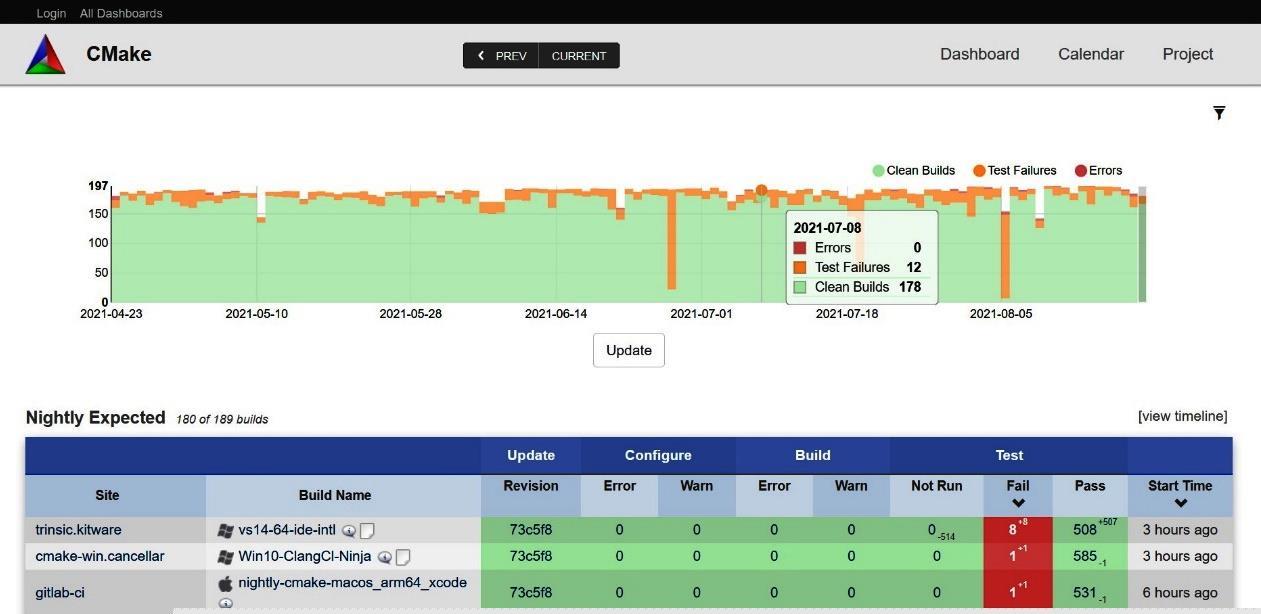
\includegraphics[width=0.8\textwidth]{content/3/chapter8/images/1.jpg}\\
Figure 8.1 ‒ Screenshot of the CDash dashboard timeline view
\end{center}

CDash isn't in the scope of this book since it's an advanced solution used as a shared server, accessible for all developers in a company.

\begin{tcolorbox}[colback=blue!5!white,colframe=blue!75!black,title=Note]
If you're interested in learning more online, reference the official documentation of CMake and visit the CDash website:

\url{https://cmake.org/cmake/help/latest/manual/ctest.1.html\#dashboard-client}

\url{https://www.cdash.org/}
\end{tcolorbox}

Let's get back to the first two modes. The command line for test mode looks like this:

\begin{tcblisting}{commandshell={}}
ctest [<options>]
\end{tcblisting}

In this mode, CTest should be executed in the build tree, after building the project with cmake. This is slightly cumbersome during the development cycle, as you'd need to execute multiple commands and change the working directory back and forth. To simplify the process, CTest added a second mode: build-and-test mode.

\subsubsubsection{8.3.1\hspace{0.2cm}Build-and-test mode}

To use this mode, we need to execute ctest starting with -{}-build-and-test, as follows:

\begin{tcblisting}{commandshell={}}
ctest --build-and-test <path-to-source> <path-to-build>
      --build-generator <generator> [<options>...]
      [--build-options <opts>...]
      [--test-command <command> [<args>...]]
\end{tcblisting}

Essentially, this is a simple wrapper around the regular test mode that accepts a few build configuration options and allows us to append the command for the first mode— in other words, all options that can be passed to ctest <options> will work when passed to ctest --build-and-test. The only requirement here is to pass the full command after the -{}-test-command argument. Contrary to what you might think, build-and-test mode won't actually run any tests unless provided with ctest keyword after -{}-testcommand, like so:

\begin{tcblisting}{commandshell={}}
ctest --build-and-test project/source-tree /tmp/build-tree
--build-generator "Unix Makefiles" --test-command ctest
\end{tcblisting}

In this command, we specify source and build paths, and select a build generator. All three are required and follow the rules for the cmake command, described in detail in Chapter 1, First Steps with CMake.

You may pass additional arguments to this mode. They come in three groups, controlling the configuration, the build process, or the tests.

Here are the arguments for controlling the configuration stage:

\begin{itemize}
\item 
-{}-build-options—Any extra options for the cmake configuration (not the build tool) should be provided just before -{}-test-command, which comes last.

\item 
-{}-build-two-config—Run the configuration stage for CMake twice.

\item 
-{}-build-nocmake—Skip the configuration stage.

\item 
-{}-build-generator-platform, --build-generator-toolset— Provide a generator-specific platform and toolset.

\item 
-{}-build-makeprogram—Specify a make executable when using Make- or Ninja-based generators.
\end{itemize}

Here are the arguments for controlling the build stage:

\begin{itemize}
\item 
-{}-build-target—Build the specified target (instead of the all target).
	
\item 
-{}-build-noclean—Build without building the clean target first.
	
\item 
-{}-build-project—Provide the name of the built project.
\end{itemize}

This is the argument used to control the test stage:

\begin{itemize}
\item 
-{}-test-timeout—Limit the execution of tests (provided in seconds).
\end{itemize}

All that's left is to configure the regular testing mode after the -{}-test-command cmake argument.

\subsubsubsection{8.3.2\hspace{0.2cm}Test mode}

Assuming that we have built our project and we're executing ctest in the build tree (or we're using the build-and-test wrapper), we can finally execute our tests.

A simple ctest command without any arguments is usually enough to get satisfactory results in most scenarios. If all tests pass, ctest will return a 0 exit code. Use this in your CI/CD pipeline to prevent faulty commits from merging to your repository's production branch.

Writing good tests can be as challenging as writing the production code itself. We set up our SUT to be in a specific state, run a single test, and then tear down the SUT instance. This process is rather complex and can generate all sorts of issues: cross-test pollution, temporal and concurrency disruptions, resource contention, frozen execution due to deadlocks, and many others.

We can employ strategies that help detect and solve some of these problems. CTest allows you to affect test selection, their order, produced output, time limits, repetition, and so on. The following sections will provide the necessary context and a brief overview of the most useful options. As always, refer to the CMake documentation for an exhaustive list.

\hspace*{\fill} \\ %插入空行
\noindent
\textbf{Querying tests}

The first thing we might need to do is to understand which tests are actually written for the project. CTest offers an -N option, which disables execution and only prints a list, as follows:

\begin{tcblisting}{commandshell={}}
# ctest -N
Test project /tmp/b
  Test #1: SumAddsTwoInts
  Test #2: MultiplyMultipliesTwoInts
Total Tests: 2
\end{tcblisting}

You might want to use -N with the filters described in the next section to check which tests would be executed when a filter is applied.

If you need a JSON format that can be consumed by automated tooling, execute ctest with --show-only=json-v1.

CTest also offers a mechanism to group tests with LABELS keyword. To list all available labels (without actually executing any tests), use -{}-print-labels. This option is helpful when tests are defined manually with the add\_test(<name> <testcommand>) command in your listfile, as you are then able to specify individual labels through test properties, like this:

\begin{lstlisting}[style=styleCMake]
set_tests_properties(<name> PROPERTIES LABELS "<label>")
\end{lstlisting} 

On the other hand, the frameworks we'll discuss later provide automatic test discovery, which unfortunately doesn't support such a granular level of labeling yet.

\hspace*{\fill} \\ %插入空行
\noindent
\textbf{Filtering tests}

There are plenty of reasons to run only a subset of all tests—the most common one might be the need to debug a single failing test or a module you're working on. There's no point in waiting for all other tests in that case. Other advanced testing scenarios will even go as far as partitioning test cases and distributing the load across a fleet of test runners.

These flags will filter tests according to the provided <r> regular expression (regex), as follows:

\begin{itemize}
\item 
-R <r>, -{}-tests-regex <r>—Only run tests with names matching <r>

\item 
-E <r>, -{}-exclude-regex <r>—Skip tests with names matching <r>

\item 
-L <r>, -{}-label-regex <r>—Only run tests with labels matching <r>

\item 
-LE <r>, -{}-label-exclude <regex>—Skip tests with labels matching <r>
\end{itemize}

Advanced scenarios can be achieved with the -{}-tests-information option (or the shorter form, -I). Use this filter to provide a range in a comma-separated format: <start>, <end>, <step>. Any of the fields can be empty, and after one more comma, you can append individual <test-id> values to run them additionally. Here are some examples:

\begin{itemize}
\item 
-I 3,, will skip tests 1 and 2 (execution starts from the third test)

\item 
-I ,2, will only run the first and second test

\item 
-I 2,,3 will run every third test, starting from the second test in the row

\item 
-I ,0,,3,9,7 will only run the third, ninth, and seventh test
\end{itemize}

Optionally, CTest will accept the filename containing the specification in the same format. As you might imagine, users prefer filtering tests by name. This option can be used to distribute tests across multiple machines for really large suites.

By default, the -I option used with -R will narrow the execution (only tests matching both requirements will run). Add the -U option if you need the union of the two to execute instead (any of the requirements will suffice).

As mentioned before, you can use the -N option to check the outcome of filtering.

\hspace*{\fill} \\ %插入空行
\noindent
\textbf{Shuffling tests}

Writing unit tests can be tricky. One of the more surprising problems to encounter is test coupling, which is a situation where one test affects another by incompletely setting or clearing the state of SUT. In other words, the first test to execute can "leak" its state and pollute the second test. Such coupling is bad news because it introduces unknown, implicit relations between tests.

What's worse, this kind of error is known to hide really well in the complexities of testing scenarios. We might detect it when it causes one of the tests to fail when it shouldn't, but the opposite is equally possible: an incorrect state causes the test to pass when it shouldn't. Such falsely passing tests give developers an illusion of security, which is even worse than not having tests at all. The assumption that the code is correctly tested may encourage bolder actions, leading to unexpected outcomes.

One way of discovering such problems is by running each test in isolation. Usually, this is not the case when executing test runners straight from the testing framework without CTest. To run a single test, you'll need to pass a framework-specific argument to the test executable. This allows you to detect tests that are passing in the suite but are failing when executed on their own.

CTest, on the other hand, effectively removes all memory-based cross-contamination of tests by implicitly executing every test case in a child CTest instance. You may even go further and add the -{}-force-new-ctest-process option to enforce separate processes.

Unfortunately, this alone won't work if your tests are using external, contested resources such as GPUs, databases, or files. An additional precaution we can take is to simply randomize the order of test execution. Such disturbance is often enough to eventually detect such spuriously passing tests. CTest supports this strategy with the --schedulerandom option.

\hspace*{\fill} \\ %插入空行
\noindent
\textbf{Handling failures}

Here's a famous quote from John C. Maxwell: "Fail early, fail often, but always fail forward." This is exactly what we want to do when running unit tests (and perhaps in other areas of life). Unless you're running your tests with a debugger attached, it's not easy to learn where you made a mistake as CTest will keep things brief and only list tests that failed, without actually printing any of their output.

Messages printed to stdout by the test case or the SUT might be invaluable to determine what was wrong exactly. To see them, we can run ctest with -{}-output-on-failure. Alternatively, setting the CTEST\_OUTPUT\_ON\_FAILURE environment variable will have the same effect.

Depending on the size of the solution, it might make sense to stop execution after any of the tests fail. This can be done by providing the -{}-stop-on-failure argument to ctest.

CTest stores the names of failed tests. In order to save time in lengthy test suites, we can focus on these failed tests and skip running the passing tests until the problem is solved.

This feature is enabled with the -{}-rerun-failed option (any other filters will be ignored). Remember to run all tests after solving all issues to make sure that no regression has been introduced in the meantime.

When CTest doesn't detect any tests, it may mean two things: either tests aren't there or there's an issue with the project. By default, ctest will print a warning message and return a 0 exit code, to avoid muddying the waters. Most users will have enough context to understand which case they encountered and what to do next. However, in some environments, ctest will be executed always, as part of an automated pipeline.

Then, we might need to explicitly say that a lack of tests should be interpreted as an error (and return a nonzero exit code). We can configure this behavior by providing the -{}-no-tests=error argument. For the opposite behavior (no warning), use the -{}-no-tests=ignore option.

\hspace*{\fill} \\ %插入空行
\noindent
\textbf{Repeating tests}

Sooner or later in your career, you'll encounter tests that work correctly most of the time. I want to emphasize the word most. Once in a blue moon, these tests will fail for environmental reasons: because of incorrectly mocked time, issues with event loops, poor handling of asynchronous execution, parallelism, hash collisions, and other really complicated scenarios that don't occur on every run. These unreliable tests are called "flaky tests".

Such inconsistency seems a not-so-important problem. We might say that tests aren't a real production environment and this is the ultimate reason why they sometimes fail. There is a grain of truth in this: tests aren't meant to replicate every little detail, because it's not viable. Tests are a simulation, an approximation of what might happen, and that's usually good enough. Does it hurt to rerun tests if they'll pass on the next execution?

Actually, it does. There are three main concerns, as outlined here:

\begin{itemize}
\item 
If you have gathered enough flaky tests in your code base, they will become a serious obstacle to the smooth delivery of code changes. It's especially frustrating when you're in a hurry: either getting ready to go home on a Friday afternoon or delivering a critical fix to a severe issue impacting your customers.

\item 
You can't be truly sure that your flaky tests are failing because of the inadequacy of the testing environment. It may be the opposite: they fail because they replicated a rare scenario that already occurs in production. It's just not obvious enough to raise an alert… yet.

\item 
It's not the test that's flaky—it's your code! The environment is wonky from time to time—as programmers, we deal with that in a deterministic manner. If SUT behaves this way, it's a sign of a serious error—for example, the code might be reading from uninitialized memory.
\end{itemize}

There isn't a perfect way to address all of the preceding cases—the multitude of possible reasons is simply too great. However, we might increase our chance of identifying flaky tests by running them repeatedly with the –repeat <mode>:<\#> option. Three modes are available, as outlined here:

\begin{itemize}
\item 
until-fail—Run test <\#> times; all runs have to pass.

\item 
until-pass—Run test up to <\#> times; it has to pass at least once. This is useful when dealing with tests that are known to be flaky, but too difficult and important to debug or disable.

\item 
after-timeout—Run test up to <\#> times but retry only if the test is timing out. Use it in busy test environments.
\end{itemize}

A general recommendation is to debug flaky tests as quickly as possible or get rid of them if they can't be trusted to produce consistent results.

\hspace*{\fill} \\ %插入空行
\noindent
\textbf{Controlling output}

Printing every piece of information to the screen every time would instantly get incredibly busy. CTest reduces the noise and collects the outputs of tests it executes to the log files, providing only the most useful information on regular runs. When things go bad and tests fail, you can expect a summary and possibly some logs if you enabled --output-onfailure, as mentioned earlier.

I know from experience that "enough information" is enough until it isn't. Sometimes, we may want to see the output of passed tests too, perhaps to check if they're truly working (and not just silently stopping without an error). To get access to more verbose output, add the -V option (or -{}-verbose if you want to be explicit in your automated pipelines).

If that's not enough, you might want -VV or -{}-extra-verbose. For extremely in-depth debugging, use -{}-debug (but be prepared for walls of text with all the details). If you're looking for the opposite, CTest also offers "Zen mode" enabled with -Q, or -{}-quiet. No output will be printed then (you can stop worrying and learn to love the calm). It seems that this option has no other use than to confuse people, but be aware that the output will still be stored in test files (in ./Testing/Temporary by default). Automated pipelines can check if the exit code is a nonzero value and collect the log files for further processing without littering the main output with details that may confuse developers not familiar with the product.

To store the logs in a specific path, use the -O <file>, -{}-output-log <file> option. If you're suffering from lengthy outputs, there are two limit options to cap them to the given number of bytes per test: -{}-test-output-size-passed <size> and -{}-test-output-size-failed <size>.

\hspace*{\fill} \\ %插入空行
\noindent
\textbf{Miscellaneous}

There are a few other useful options that can be useful for your everyday testing needs, as outlined here:

\begin{itemize}
\item 
-C <cfg>, -{}-build-config <cfg> (multi-configuration generators only)— Use this to specify which configuration to test. The Debug configuration usually has debugging symbols, making things easier to understand, but Release should be tested too, as heavy optimization options could potentially affect the behavior of SUT.

\item 
-j <jobs>, -{}-parallel <jobs>—This sets the number of tests executed in parallel. It's very useful to speed up the execution of long tests during development. Be mindful that in a busy environment (on a shared test runner), it might have an adverse effect due to scheduling. This can be slightly mitigated with the next option

\item 
-{}-test-load <level>—Use this to schedule parallel tests in a fashion that CPU load doesn't exceed the <level> value (on a best-effort basis).

\item 
-{}-timeout <seconds>—Use this to specify the default limit of time for a single test.
\end{itemize}

Now that we understand how to execute ctest in many different scenarios, let's learn how to add a simple test.


























